\section{Object Selection Criteria}
\label{sec:criteria}
\subsection{Overview}
{\color{red}Some words that introduce the section. What do we do here? Calculate completeness and contamination for various color cuts.  Re-emphasize that the extragalactic sources are not in the region of the LMC, so we estimate their numbers (and thus the contamination fraction) by scaling their number density per square degree up by the space occupied by the LMC. Then we add some more color cuts to reject YSOs. We should also do something with O-rich and C-rich criteria from Nikutta et al 2014, however it does use W4 which we neglect.}

\subsection{Completeness and Contamination of Initial Samples}
Sample completeness $\eta$ is defined as
\begin{eqnarray*}
\eta &=& \frac{N - n_\text{missed}}{N}
\end{eqnarray*}
where $N$ is the total number of objects in the sample, and $n_\text{missed}$ is the number of objects outside of the applied boundaries. \cite{2013sdmm.book.....I} defines sample contamination as
\begin{eqnarray*}
\epsilon &=& \frac{n_\text{spurious}}{n_\text{selected}}.
\end{eqnarray*}
where $n_\text{spurious}$ is the number of spurious sources and $n_\text{selected} = N + n_\text{spurious}$. Our goal is to get the lowest AGB sample ($\le$1\% contamination) while still retaining a large number of AGB stars.

The difficulty with determining contamination is that none of the contaminant sample, save for the locus stars,  falls within the region occupied by our AGB sample: the LMC. However, knowing that there is essentially a uniform distribution of extragalactic sources on the sky {\color{red}[a citation would be great]}, we solve for the number density of objects in the 10,417 sq. deg. DR7 footprint. We then scale these number densities up by the $\sim76.5$ deg$^2$ area occupied by the LMC. This should provide a reasonable estimate for the number of sources that we would find within the region of the LMC, and by consequence estimate our final levels of extragalactic contamination in WISE-2MASS color-color space. 

We employ the following color criteria to isolate AGB stars from their potential contaminants:
\begin{eqnarray}
(J - K_s) &>& 1.1\\
(W2 - W3) &<&  2.2
\end{eqnarray}
\noindent Figure~\ref{fig:colorcuts} shows completeness distributions for the OGLE-2MASS-WISE AGB sample, and corresponding contamination distributions for each contaminant sample. Tables~\ref{tab:criteria_completeness} \&~\ref{tab:criteria_contamination} show the completeness and contamination fractions for each color criterion. 

\begin{figure}[h]
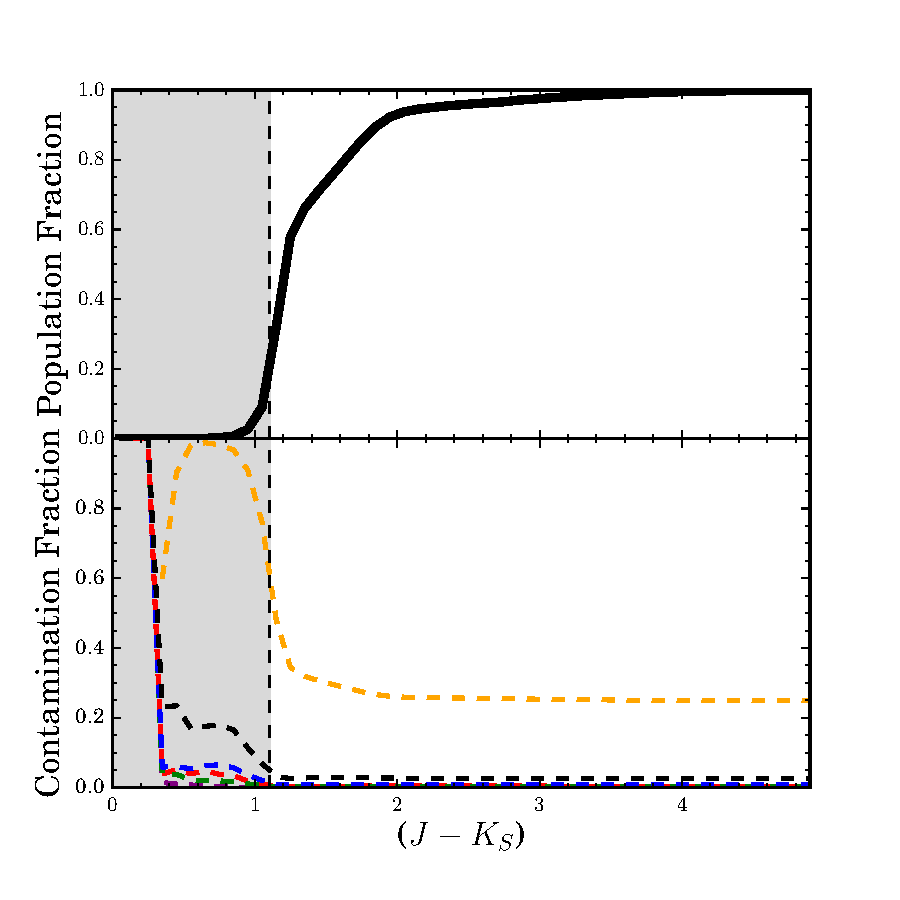
\includegraphics[width=3.3in]{figs/completeness_contamination_jkcut.pdf}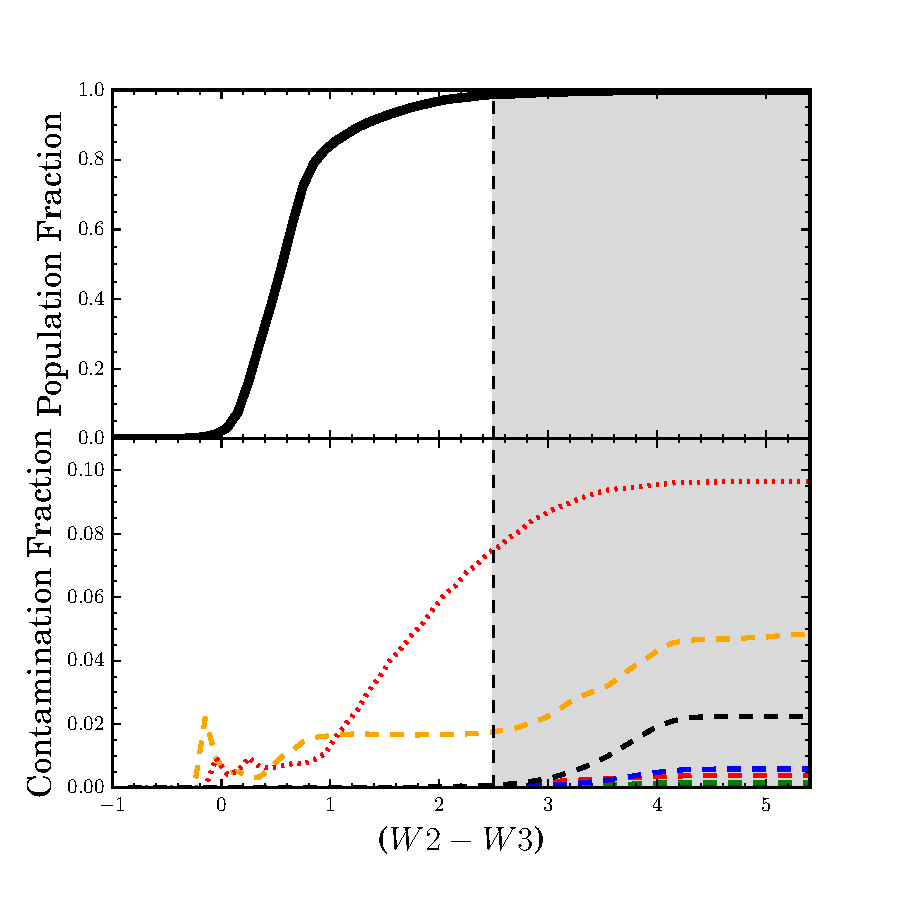
\includegraphics[width=3.3in]{figs/completeness_contamination_w23cut.pdf}
\caption{\emph{Left:} Cumulative completeness and contamination distributions before $(J-K_s)$ color cut. \emph{Right:} Cumulative completeness and contamination after $(J-K_s)$ cut and before $(W2-W3)$ cuts. Colors are the same as Figure~\ref{fig:wisecontaminants}. Thick black line in top panels is OGLE-2MASS-WISE AGB completeness as a function of color. Bin width for both panels is 0.1 dex. \label{fig:colorcuts}}
\end{figure}

\begin{table}[h]
	\begin{center}
	\scalebox{0.85}{
		\begin{tabular}{l r r r}
		\hline\hline
		Criteria & Completness \\
		\hline
		$(J-K_s) > 1.1$ & 89.62\%\\
		$(W2-W3) < 2.2$ & 82.40\%\\
		\hline\hline
		\end{tabular}}    
	\caption{Sample completeness with respect to each successive cut on WISE-2MASS color.\label{tab:criteria_completeness}}
	\end{center}
	
\end{table}
\begin{table}[h]
	\begin{center}
	\scalebox{0.85}{		
		\begin{tabular}{l r r r r r r r r}
		\hline\hline
		Critiera & QSO & AGN & LRG & SF & SB & Locus \\
		\hline
		$(J-K_s) > 1.1$ & 0.18\% & 0.09 \%& 0.04\% & 0.18\% & 0.31\% & 2.26\%\\
		$(W2-W3) < 2.2$ & 0\% & 0\%& 0.01\% & 0\% & 0\% & 0.83\%\\
		\hline\hline
		\end{tabular}
		}    
	\caption{Sample contamination with respect to each successive cut on WISE-2MASS color.\label{tab:criteria_contamination}}
	\end{center}
\end{table}

Figure~\ref{fig:lmc_completeness} shows the distribution of recovered AGB stars on the sky as well as in color-color space. We reserve an accounting of YSOs for the next section, as there is significant overlap between YSOs and AGBs, and they are not evenly distributed across the sky.

\begin{figure}[h]
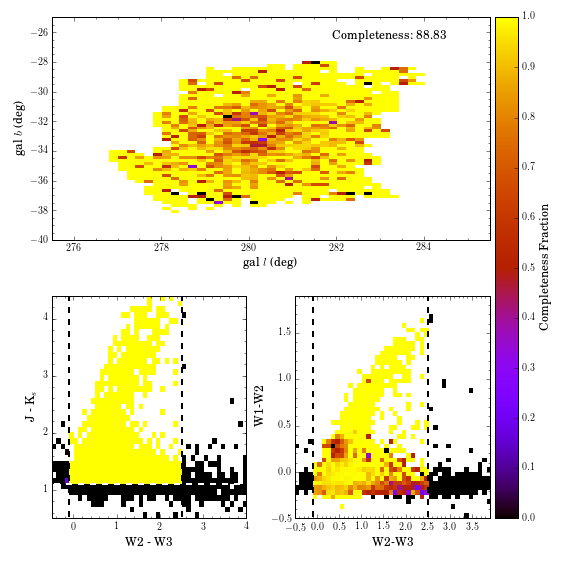
\includegraphics[width=6in]{figs/ogle_completeness_map.png}
\caption{Map of completeness fractions for AGB stars in the LMC \label{fig:lmc_completeness}}
\end{figure}

\subsection{Accounting for YSOs}
{\color{red}Talk about how you reject YSOs}


%In creating color-color criteria to generate a catalog of AGB candidates, we seek to maximize AGB completeness while minimizing contamination from non-AGB objects to beneath the 1\% level.
%
%The color-color criteria for AGB selection are as follows:
%\begin{align} 
%	(J-K_s) > 1.1\label{eq:criteria1}\\
%	(W2-W3) > 0.3\label{eq:criteria2}\\
%	(W3-W4) < -0.83(W2-W3) + 3.37\label{eq:criteria3}
%\end{align}
%The criteria in (\ref{eq:criteria1}) and (\ref{eq:criteria2}) are primarily concerned with rejecting objects from the stellar locus, and other objects whose NIR spectra are dominated by the Rayleigh-Jeans tail. (\ref{eq:criteria3}) also rejects stars from the stellar locus, but primarily functions to remove IR-bright extragalactic sources.
%
%We also experiment with other criteria to focus more closely on the high-reliability AGB population, instead of trying to capture the most AGB-like objects. These criteria are as follows:
%\begin{align} 
%	(W1-W2) < 1\label{eq:criteria4}\\
%	(W2-W3) < 1\label{eq:criteria5}
%\end{align}
%Criteria (\ref{eq:critera4}) restricts NIR excesses. Criteria (\ref{eq:criteria5}) primarily removes extragalactic sources, while only slightly cutting into the distribution of known AGB stars.
%
%\noindent Sample completeness $\eta$ is defined as
%\begin{eqnarray*}
%\eta &=& \frac{N - n_\text{missed}}{N}
%\end{eqnarray*}
%where $N$ is the total number of objects in the sample, and $n_\text{missed}$ is the number of objects outside of the applied boundaries. Figure~\ref{fig:completeness} shows the distribution of sample completeness amongst AGB sources after the application of the above criteria. The vast majority (79.07\%) of Galactic AGB stars is recovered after criteria (\ref{eq:criteria1}), (\ref{eq:criteria2}), and (\ref{eq:criteria3}) are applied. The largest losses occur at the edges of the Galactic disk ($\lvert b\rvert\approx10^\circ$) and in regions of high stellar number density both in the Galaxy and the Magellanic Clouds. In the color-color diagrams, selection completeness degrades near the borders of the selection area, as objects that straddle these boundaries may exhibit enough emission in other color-color spaces to be removed by our criteria. Of the remaining sample of 5,709 objects, 52.94\% lie within the disk ($\lvert b\rvert<10^\circ$).
%
%\begin{table}[h]
%    \begin{center}
%        \caption{Samples Recovered wih Application of Criteria (\%)}
%        \scalebox{0.85}{
%            \begin{tabular}{l r r r r r r r r r r r r}
%\hline
%Object Type & Reduced & (1) & (2) & (3) & (1,2) & (1,2,3) & | & \textbf{(4)} & \textbf{(5)} & \textbf{(1,2,4)} & \textbf{(1,2,5)} & \textbf{(1,2,4,5)}\\
%\hline
%All AGBs & 7220 & 95.15 & 84.89 & 95.21 & 82.62 & 79.07 & | & \textbf{94.22} & \textbf{88.82} & \textbf{77.05} & \textbf{72.71} & \textbf{71.14}\\ 
%O-rich AGB & 3147 & 98.98 & 100.00 & 100.00 & 98.98 & 98.98 & | & \textbf{98.44} & \textbf{97.33} & \textbf{97.43} & \textbf{96.31} & \textbf{94.88}\\ 
%C-rich AGB & 540 & 99.26 & 99.81 & 99.26 & 99.07 & 98.33 & | & \textbf{57.59} & \textbf{63.33} & \textbf{56.85} & \textbf{62.59} & \textbf{54.44}\\ 
%Unclassed AGB & 3533 & 91.11 & 69.15 & 90.32 & 65.53 & 58.39 & | & \textbf{96.07} & \textbf{85.14} & \textbf{61.99} & \textbf{53.24} & \textbf{52.53}\\ 
%DR12 SSPP & 67508 & 76.16 & 99.16 & 0.91 & 76.07 & 0.05 & | & \textbf{86.05} & \textbf{0.89} & \textbf{65.67} & \textbf{0.03} & \textbf{0.03}\\ 
%DR7 LRG & 84 & 96.43 & 100.00 & 0.00 & 96.43 & 0.00 & | & \textbf{89.29} & \textbf{0.00} & \textbf{85.71} & \textbf{0.00} & \textbf{0.00}\\ 
%QSO & 3783 & 73.54 & 99.97 & 0.13 & 73.54 & 0.11 & | & \textbf{34.50} & \textbf{0.11} & \textbf{27.54} & \textbf{0.08} & \textbf{0.08}\\ 
%Galaxy & 42066 & 78.55 & 100.00 & 0.01 & 78.54 & 0.00 & | & \textbf{96.39} & \textbf{0.01} & \textbf{75.31} & \textbf{0.00} & \textbf{0.00}\\ 
%AGN & 1011 & 79.33 & 100.00 & 0.00 & 79.33 & 0.00 & | & \textbf{96.34} & \textbf{0.00} & \textbf{75.87} & \textbf{0.00} & \textbf{0.00}\\ 
%
%\hline
%                \label{tab:criteria}
%            \end{tabular}}    
%    \end{center}
%\end{table}
%
%
%\begin{figure}[h]
%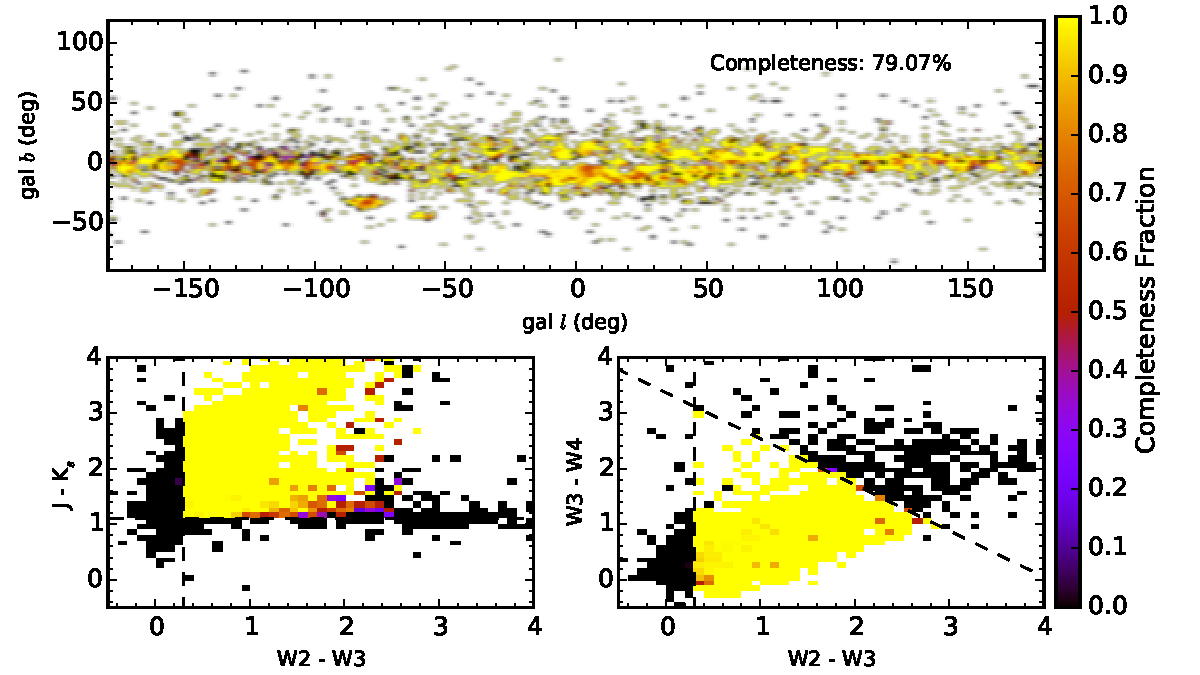
\includegraphics[width=6.7in]{figs/completeness_map.pdf}
%\caption{Sample selection completeness maps in ($l,b$) space (\emph{top}) and the color-color space of our selection criteria (\emph{bottom}). Color scale shows the completeness fraction per bin, with 4-deg$^2$ bins on the Galactic map and 0.1 dex bins on each axis of the color-color diagrams. Selection criteria are shown as dashed lines.\label{fig:completeness}}
%\end{figure}
%
%\cite{2013sdmm.book.....I} defines sample contamination as
%\begin{eqnarray*}
%\epsilon &=& \frac{n_\text{spurious}}{n_\text{selected}}.
%\end{eqnarray*}
%where $n_\text{spurious}$ is the number of spurious sources and $n_\text{selected} = N + n_\text{spurious}$. The contamination map is shown in Figure~\ref{fig:contamination}. Most bins in Figure~\ref{fig:contamination} exhibit 0\% contamination, with the overall contamination level at 0.38\%. What contaminants do remain exist primarily at the very fringes of the AGB star distribution in ($J-K_S$) vs ($W2 - W3$) space and near the redder boundary in ($W3-W4$) vs ($W2 - W3$), where bluer extragalactic sources creep into the selection region. The results of the applied criteria on both the collective AGB and contaminant samples are summarized in Table~\ref{tab:completeness}. 
%
%We note that while we do achieve a low rate of contamination, most of our contaminant sources are out of the plane of the Galaxy, while many of our \agb\, sources are within the Galactic disk. Considering how our extragalactic contaminant sources are from various iterations of \sdss, we know that their spatial distributions should be effectively uniform across the sky {\color{red} [cite me]}. For contaminants unaffected by interstellar reddening, they would occupy the same regions of color-color space already marked by our existing contaminant sample, and would similarly be removed by (\ref{eq:criteria1}), (\ref{eq:criteria2}), and (\ref{eq:criteria3}). This would produce the same zero-level contamination for all extragalactic sources aside from QSOs. We can adopt a QSO spatial density by dividing the total number of spectroscopically identified QSOs by the covered area on the sky. Using this, we recover a QSO spatial density of {\color{red} some number per square degree}. Using that density, and assuming ubiquity of sources on the sky, complete detection of QSOs {\color{red} down to some magnitude limit}, and a lack of interstellar reddening, we can estimate a maximum QSO contamination fraction of {\color{red} some number}. We use this number to report our QSO contamination fraction in Table~\ref{tab:completeness}, as QSOs significantly affected by interstellar reddening would exist further outside of the limits of (\ref{eq:criteria1}), (\ref{eq:criteria2}), and (\ref{eq:criteria3}). A more rigorous study of QSO spatial density is outside the scope of this paper.
%
%The remaining contaminant sample is from the \sdss\, DR12 SSPP, with the number of remaining species found within shown in Figure~\ref{fig:sspp_histo}. {\color{red} the figures don't match up with each other. The number of red stars on the right side of the fig are significantly less than those in the histogram. Reconcile this.}
%
%\begin{figure}[h]
%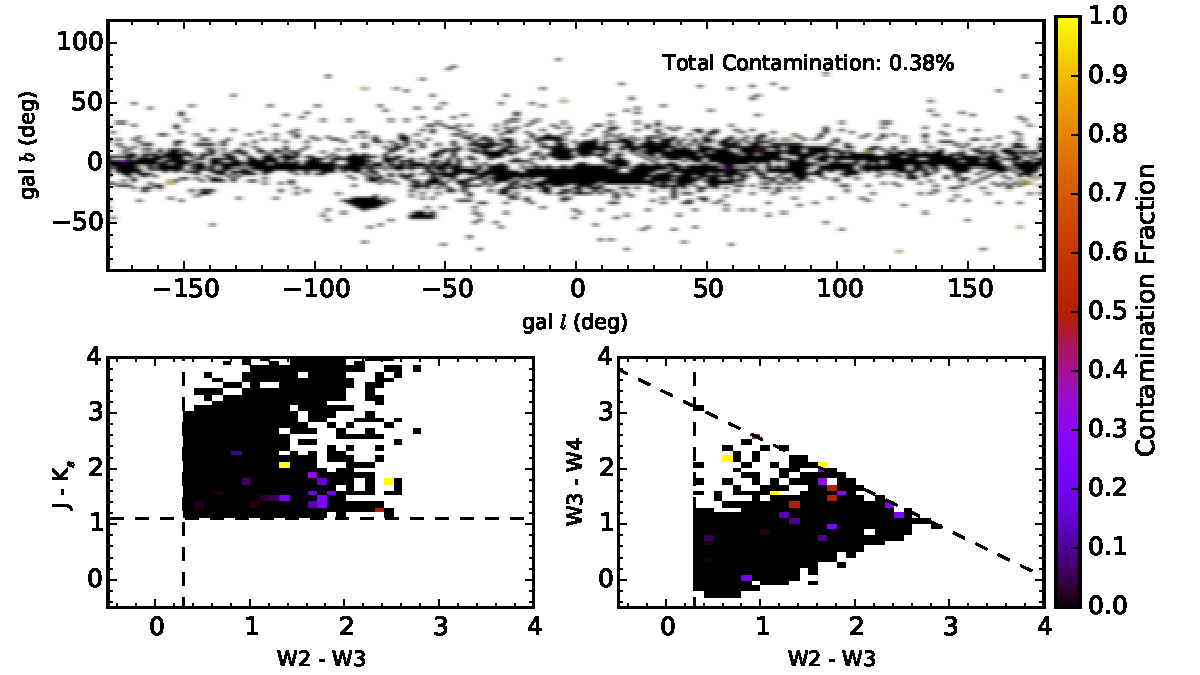
\includegraphics[width=6.7in]{figs/contamination_map.pdf}
%\caption{Sample contamination in Galactic ($l,b$) space (\emph{top}) and color-color space (\emph{bottom}). Boundaries and binning the same as Fig~\ref{fig:completeness}.\label{fig:contamination}}
%\end{figure}
%
%\begin{figure}[h]
%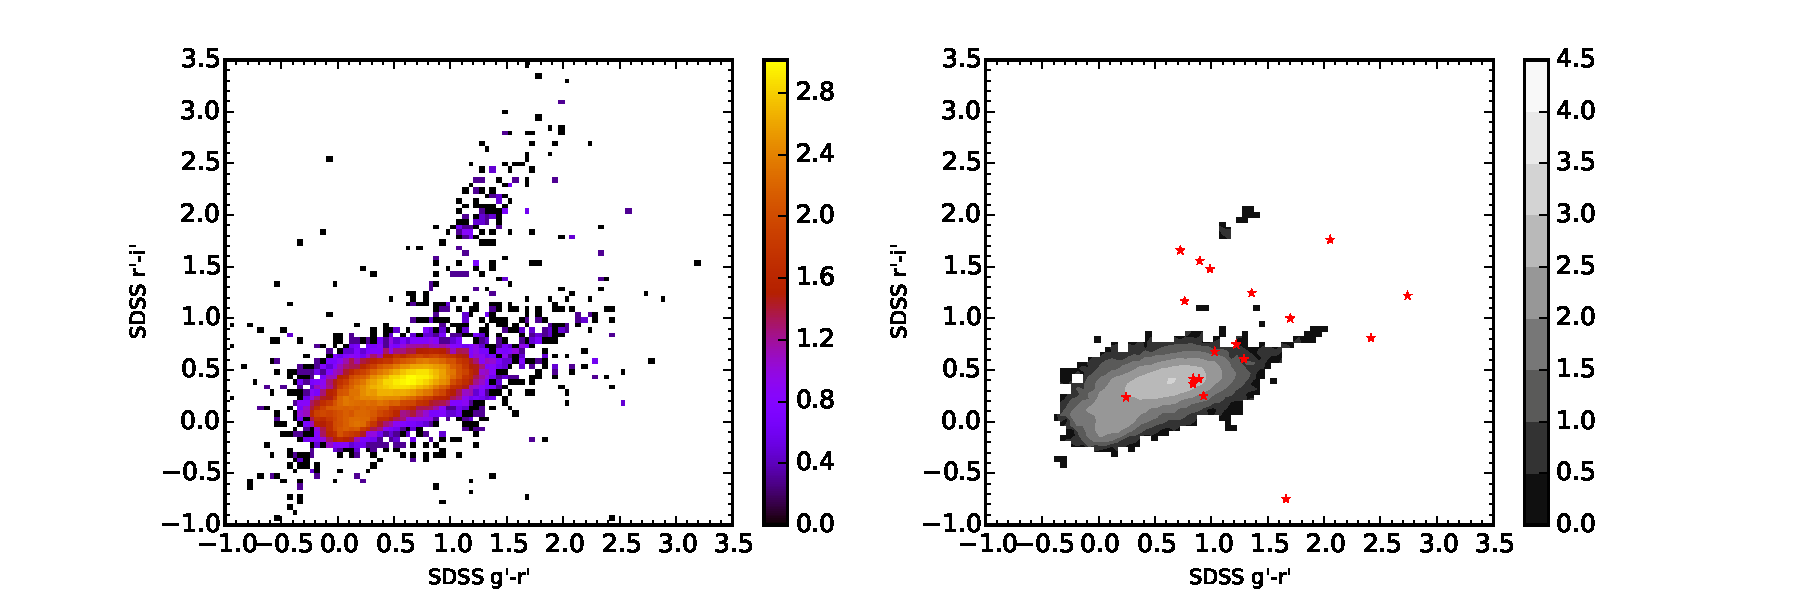
\includegraphics[width=6.7in]{figs/contaminating_sspp_objects.pdf}
%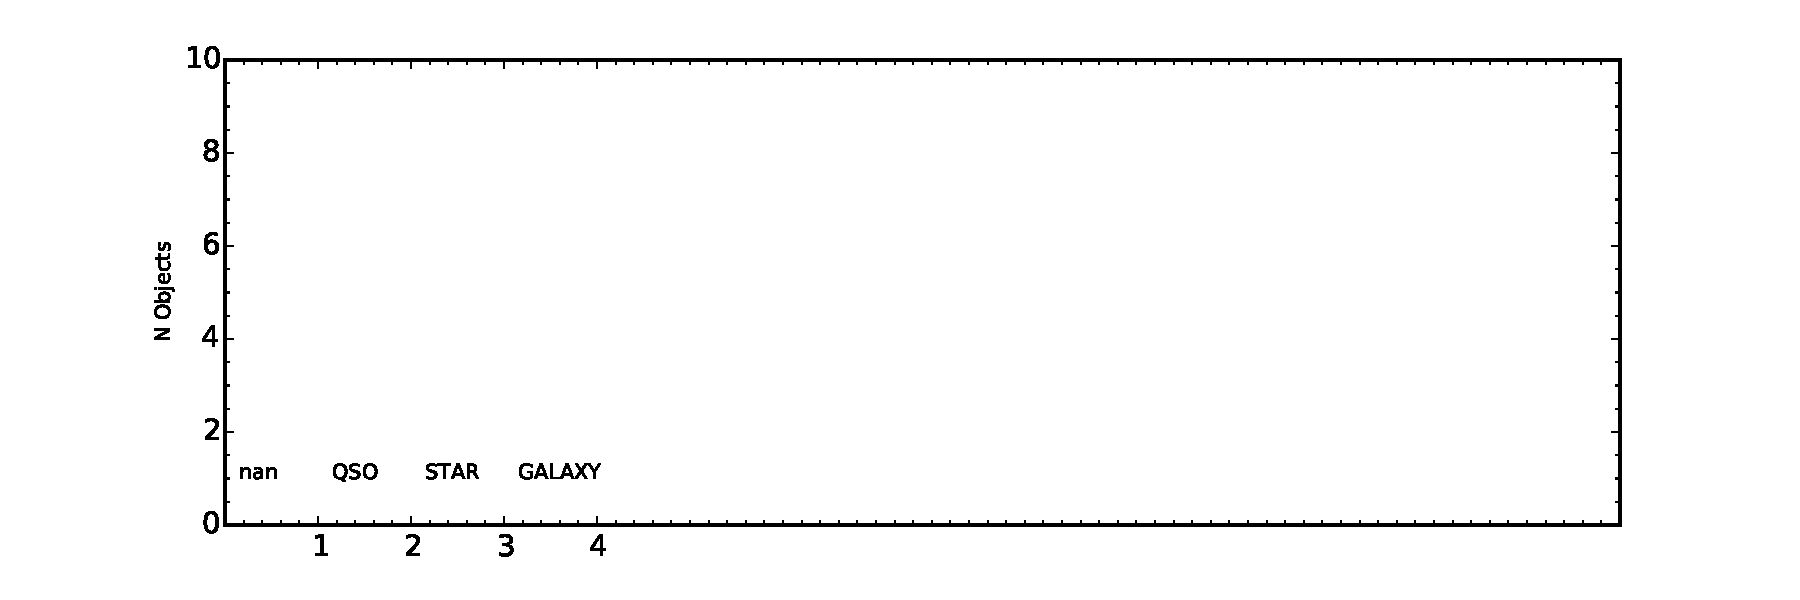
\includegraphics[width=6.7in]{figs/contaminating_sspp_objects_classes.pdf}
%\caption{Some histogram\label{fig:sspp_histo}}
%\end{figure}
%
%%One large issue with the boundaries are the O-rich AGB stars.  Either the objects from the OGLE O-rich AGB star catalog were mostly mis-matched to WISE, taking on colors of the stellar locus, or the issue is more physical.  It could be that the warm O-rich AGB photospheres are still visible and not heavily enshrouded in dust, thus appearing similar to Main Sequence stars in the NIR. Previous work on warm O-rich AGB stars has shown that their circumstellar shells are not prominent, and their NIR photometry reflects the Rayleigh Jeans tail of a cool 2000-4000K blackbody \citep{1974ApJ...189...89D}. 
%
%\begin{table}[h]
%    \begin{center}
%        \caption{Sample Selection Completeness and Contamination}
%        \scalebox{0.85}{
%            \begin{tabular}{l c c c c c c}
%		\hline
%		Population & SIMBAD AGB* & C* & Mira & OH/IR & S* \\ 
%		Completeness & 89.62\% & 72.11\% & 95.62\% & 39.53\% & 22.31\% \\ 
%		\hline
%		Population & MACHO seq1 & seq2 & seq3 & seq4 \\ 
%		Completeness & 88.45\% & 81.08\% & 28.77\% & 14.75\% \\ 
%		\hline
%		Population & OGLE-III C-rich & O-rich & \textbf{All AGB Stars} \\ 
%		Completeness & 73.09\% & 70.68\% & \textbf{79.07\%} \\ 
%		\hline
%		Population & DR12 SSPP & DR7 LRG & Galaxies & QSO & AGN \\ 
%		Contamination & 0.56\% & 0.00\% & 0.00\% & 0.07\% & 	0.00\% \\ 
%		\hline
%
%                \label{tab:completeness}
%            \end{tabular}}    
%    \end{center}
%\end{table}
%

